\chapter{Caratteristiche del robot}
\graphicspath{{media/1_intro}}
%\addcontentsline{toc}{chapter}{Introduzione}

% \renewcommand{\chaptermark}[1]{\markboth{\MakeUppercase{ #1}}{}}
% \chaptermark{Introduzione}

Il manipolatore SCARA è un robot con 4 gradi di libertà, formato da 4 giunti in configurazione $RRPR$\footnote{R: giunto rotoidale, P: giunto prismatico.}.

\begin{figure}[tbph!]
	\centering
	\label{fig:robor_pic}
	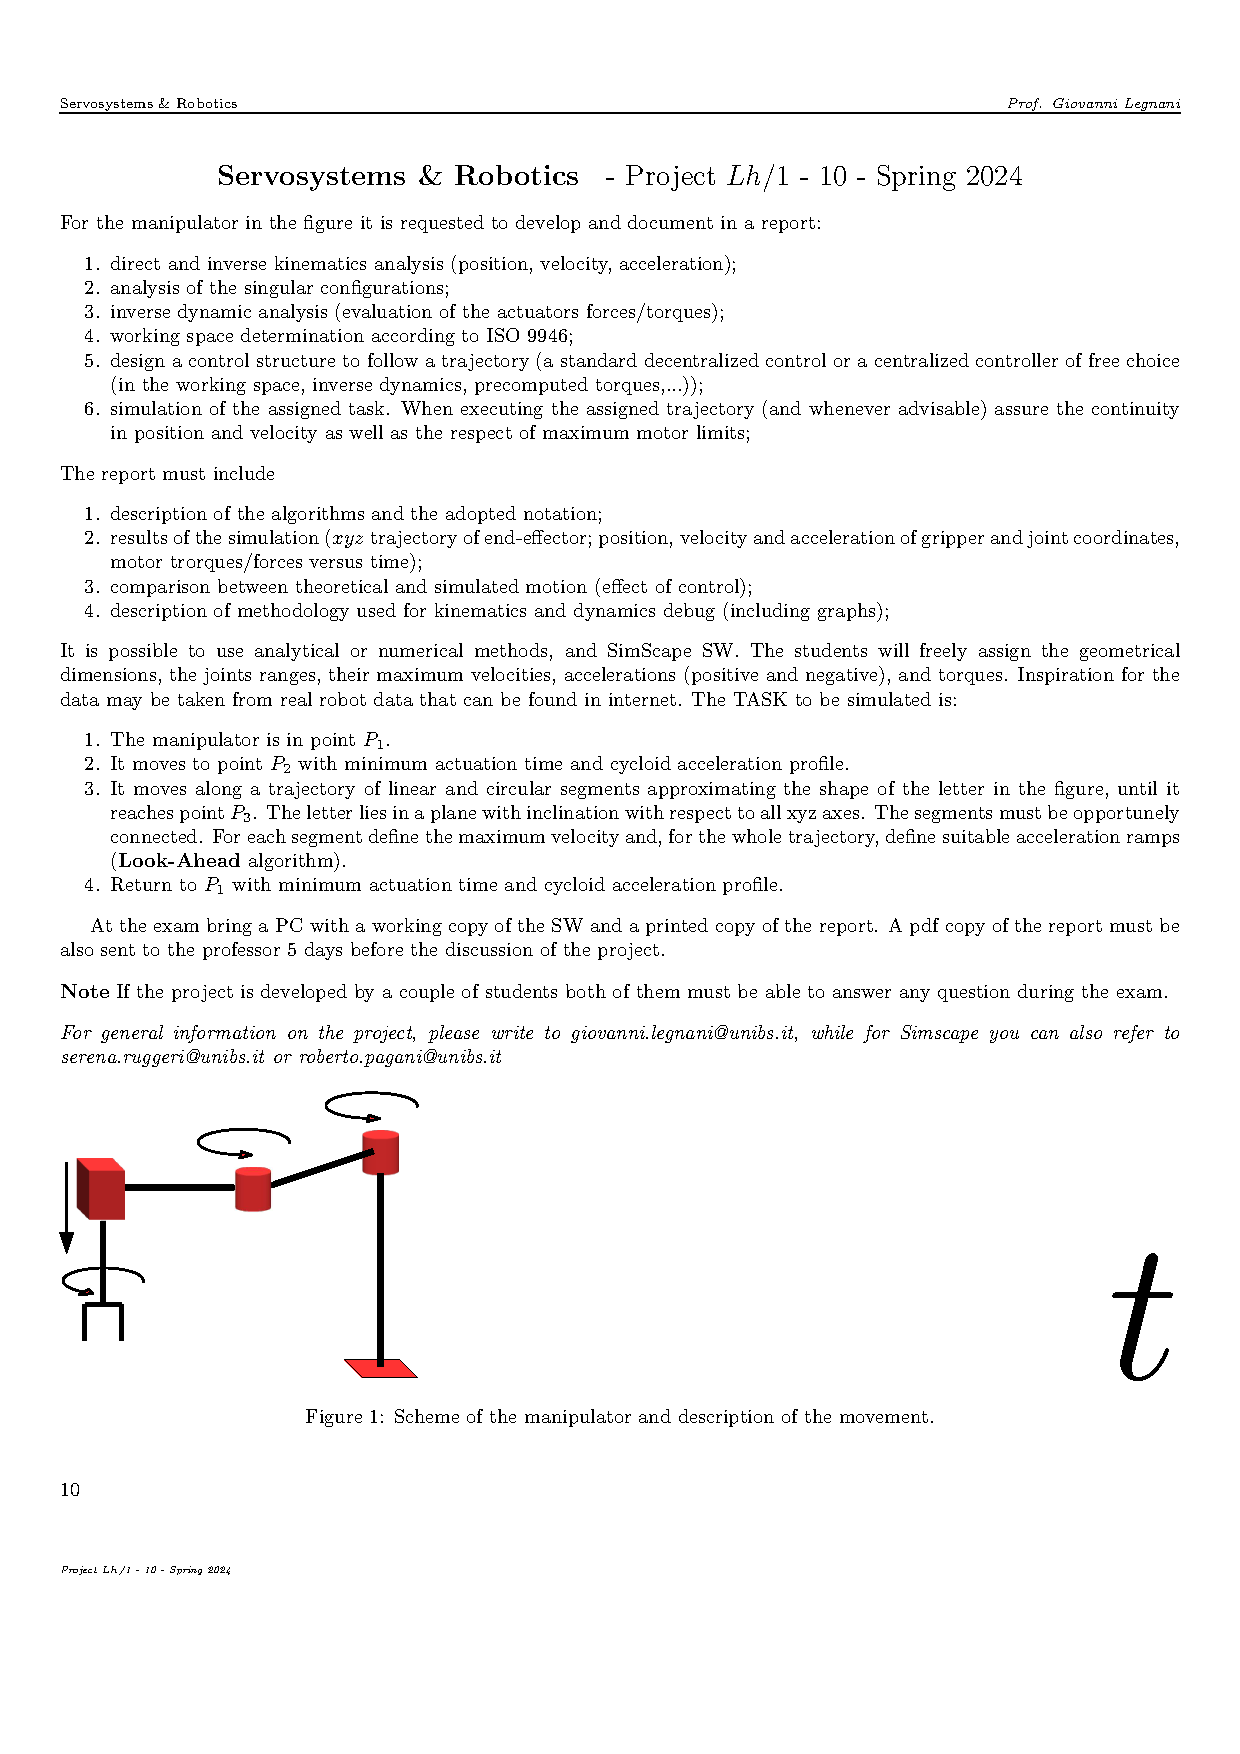
\includegraphics[trim=0 3.2cm 14cm 16cm,clip,width=0.7\linewidth]{elaborato}
	\caption{Robot SCARA.}
\end{figure}


Le masse, le inerzie, le lunghezze dei link, i limiti dell'area di lavoro, il motion range e le velocità massime dei giunti del robot sono state tratte dalla scheda tecnica di alcuni SCARA in commercio. In particolare si è considerato un esemplare Fanuc SR-20\textit{i}A, che presenta un carico massimo al polso di 20 kg e uno sbraccio massimo di 1100 mm. Si riportano nella tabella \ref{tab:caratteristiche_costruttive} i dati tecnici considerati per le simulazioni riportate nei capitoli successivi.  

\begin{table}[htbp!]
    \centering
    \begin{tabularx}{\textwidth}{Y|Y|Y}
    \hline
         \textbf{Caratteristiche giunti}  & \textbf{Motion range [°]} & \textbf{velocità max [°/s]}\\
         \hline
        Giunto 1 (R) & 290     & 440 \\
        Giunto 2 (R) & 290     & 500 \\
        Giunto 3 (P) & 300 mm  & 2800 mm/s\\
        Giunto 4 (R) & 1440    & 1700\\
        \hline
\end{tabularx}
\begin{tabularx}{\textwidth}{Y|Y|Y|Y}
     \textbf{Caratteristiche link} & \textbf{Lunghezza} $\boldsymbol{[mm]}$ & \textbf{Massa [kg] - \textit{inerzia} [$\boldsymbol{kgm^2}$]} & \textbf{Posizione baricentro dal link precedente}$\boldsymbol{[mm]}$ \\
     \hline
    Base & 300* & - & -\\
    Link 1 & 550 & 30* - \textit{3.0250}* & 275*\\
    Link 2 & 550 & 16* - \textit{1.6133}* & 275*\\
    Link 3 & 350 & 5* & 150*\\
    Polso & - & 2* - \textit{0.5} & 0\\
    \hline
\end{tabularx}
    \caption[Caratteristiche costruttive del manipolatore]{Tabella riassuntiva delle caratteristiche costruttive considerate per le simulazioni. I valori che riportano il simbolo * non sono riportati sulla scheda tecnica e sono valori stimati o scelti arbitrariamente.}
    \label{tab:caratteristiche_costruttive}
\end{table}

Nella presente relazione sono state definite alcune funzioni MATLAB specifiche per la tipologia di robot assegnata e utilizzate frequentemente:

\begin{itemize}
    \item per il calcolo della cinematica è stato utilizzato lo Jacobiano $J$. 

    \[J = \frac{\partial S}{\partial Q} = \begin{bmatrix}
        -l_1sin(\alpha)-l_2sin(\alpha+\beta) & -l_2sin(\alpha+\beta) & 0 & 0\\
        l_1cos(\alpha)+l_2cos(\alpha+\beta) & l_2cos(\alpha+\beta) & 0 & 0\\
        0 & 0 & -1 & 0\\
        1 & 1 & 0 & 1\\
    \end{bmatrix}\]

    Questa matrice, per comodità, è stata definita nella MATLAB function riportata di seguito.

    \lstinputlisting[language=Octave]{media/1_intro/SCARAjac.m}

    
    \item per il calcolo della cinematica è stata utilizzata la derivata $Jp$ rispetto al tempo dello Jacobiano $J$. 

    \[J_p = \frac{d}{dt} \left( \frac{\partial S}{\partial Q} \right) = \begin{bmatrix}
       -l_1cos(\alpha)\Dot{\alpha}-l_2cos(\alpha+\beta)(\Dot{\alpha}+\Dot{\beta}) & -l_2cos(\alpha+\beta)(\Dot{\alpha}+\Dot{\beta}) & 0 & 0\\
        -l_1sin(\alpha)\Dot{\alpha}-l_2sin(\alpha+\beta)(\Dot{\alpha}+\Dot{\beta}) & -l_2sin(\alpha+\beta)(\Dot{\alpha}+\Dot{\beta}) & 0 & 0\\
       0 & 0 & 0 & 0\\
       0 & 0 & 0 & 0 \\
    \end{bmatrix} \]

    Questa matrice, per comodità, è stata definita nella MATLAB function riportata di seguito.

    \lstinputlisting[language=Octave]{media/1_intro/SCARAjacP.m}

    \item nelle simulazioni è stata frequentemente utilizzata la legge di moto cicloidale:

    \lstinputlisting[language=Octave]{media/1_intro/cicloidale.m}

    \item per la definizione delle caratteristiche del robot come da tabella \ref{tab:caratteristiche_costruttive} si invoca all'inizio di ogni simulazione il seguente script:

    \lstinputlisting[language=Octave]{media/1_intro/geometria_SCARA.m}
    
\end{itemize}

Si riportano in figura \ref{fig:working_space} i grafici che mostrano l'area di lavoro del robot in accordo con la normativa UNI EN ISO 9787.

\begin{figure}[htbp!]
    \centering
    \begin{subfigure}[b]{\textwidth}
        \centering
        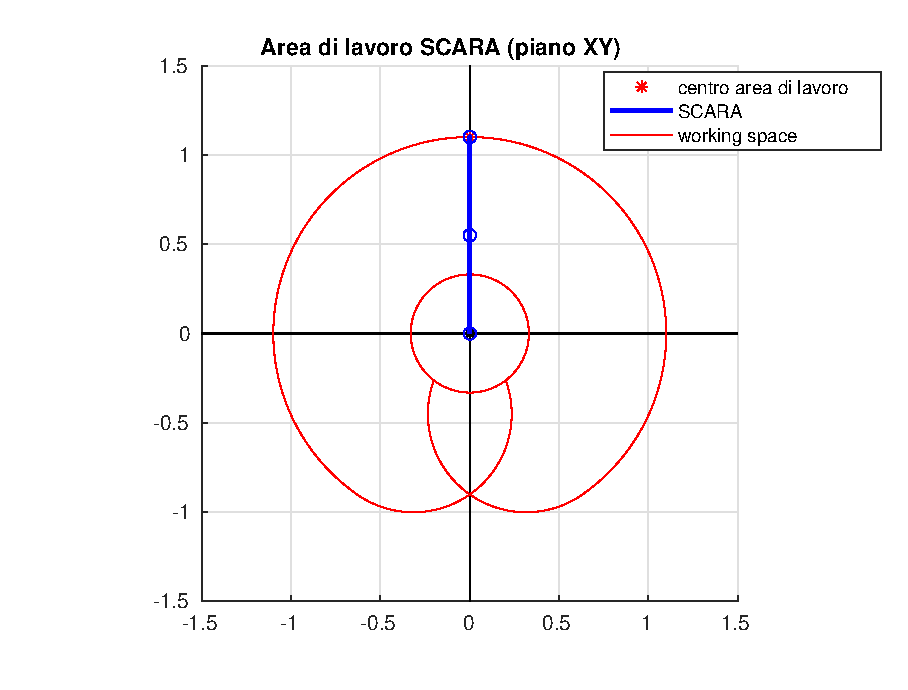
\includegraphics[width=0.8\linewidth]{working_area_xy}
        \caption{Area di lavoro SCARA - piano xy}
        \label{fig:working_space_XY}
    \end{subfigure}
    \hfill
    \begin{subfigure}[b]{\textwidth}
        \centering
        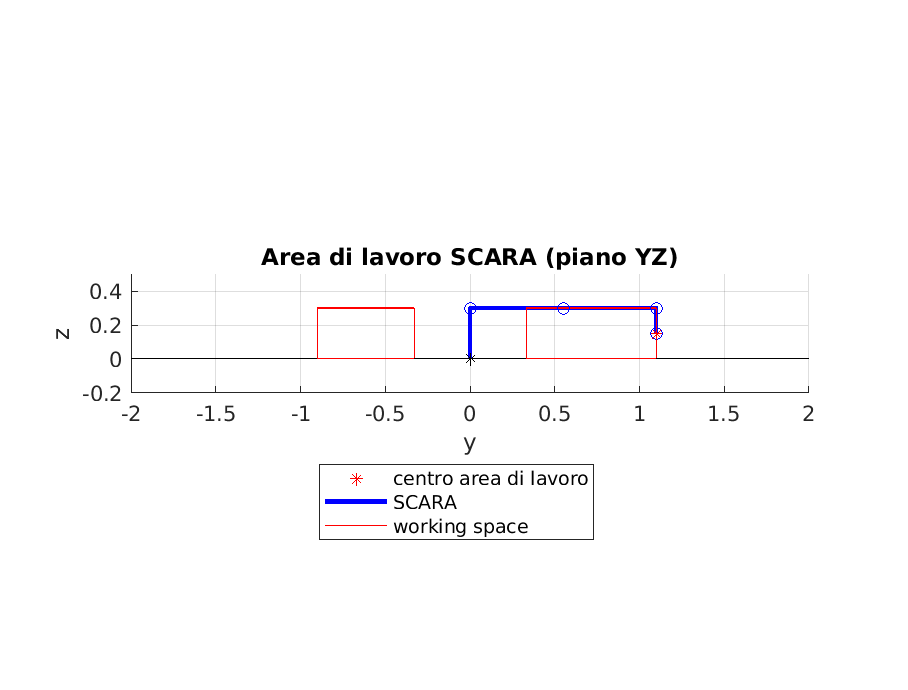
\includegraphics[width=0.8\linewidth]{working_area_yz}
        \caption{Area di lavoro SCARA - piano yz}
        \label{fig:working_space_YZ}
    \end{subfigure}
    \caption{Area di lavoro con manipolatore in una posizione singolare.}
    \label{fig:working_space}
\end{figure}

Il manipolatore presenta posizioni singolari nelle configurazioni in cui i primi due link sono allineati nello spazio. Ciò avviene quando il secondo giunto $ \beta $ assume valori pari a $ \beta = 0\degree $ oppure $ \beta = 180\degree $.

